%!TEX root = ../sbc-template.tex

A fundamentação teórica para a realização deste trabalho compreende conceitos ligados às  \emph{Smart} TVs e ao \emph{Machine Learning}. Quanto ao primeiro tópico, uma caracterização das \emph{Smart} TVs é apresentada na Subseção \ref{sec:smarttv}, e uma visão geral dos conceitos ligados à classificação indicativa é apresentada na Subseção \ref{sec:classificacaoIndicativa}. Quanto ao segundo tópico, a Subseção \ref{sec:machineLearning} compreende os conceitos essenciais de \emph{Machine Learning}, em que as redes neurais são particularmente detalhadas na Subseção \ref{sec:rnas}. Os conceitos mais emergentes desta área, envolvendo \emph{Deep Learning}, são descritos na Subseção \ref{sec:dl}.

\subsection{\emph{Smart} TVs} \label{sec:smarttv}
%!TEX root = ../sbc-template.tex

\emph{Smart} TV é tida como um aparelho de televisão com capacidades interativas ligadas à internet, como aplicativos disponíveis em lojas; acesso a conteúdo online como notícias, previsão do tempo, informações de mercados de ações, mapas e jogos; \emph{e-commerce}; navegação web e acesso a redes sociais\cite{shin2013smart}. Estes aparelhos podem ser equipadas com câmeras e microfones embutidos\cite{michele2014watch}, além de óculos 3D \cite{perakakis2015proposed}, como mostra a Figura \ref{fig:smart_samsung}. Estas televisões utilizam os mesmos sistemas operacionais e conjuntos de aplicativos que computadores comuns, o que as torna sucetíveis às mesmas falhas e ataques de segurança que outros dispositivos semelhates \cite{michele2014watch}.
\begin{figure}
	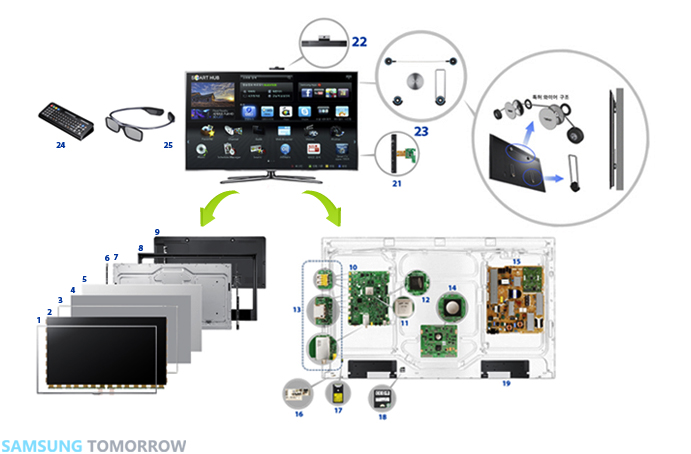
\includegraphics[width=\textwidth]{img/smart_samsung.jpg}
	\caption{\emph{Smart} TV Samsung}
	\label{fig:smart_samsung}
\end{figure}


\subsection{Classificação Indicativa para Conteúdo Televisivo} \label{sec:classificacaoIndicativa}
%!TEX root = ../../novoIndex.tex

O processo de classificação indicativa integra o sistema de garantias dos direitos da criança e do adolescente quanto a promover, defender e garantir o acesso a espetáculos e diversões públicas adequados à condição de seu desenvolvimento, mas reserva-se o direito final aos pais e responsáveis quanto à escolha do conteúdo adequado a estes \cite{eca}.


%!TEX root = ../../novoIndex.tex
\begin{table}[!ht]
  \scalefont{0.8}
  \caption{Categorias de classificação indicativa propostas pela Portaria No. 368, de 11 de Fevereiro de 2014. Fonte: \cite{ci:guia}}
  \label{tab:categorias}
	\centering
	\begin{tabular}{p{4cm} p{1.5cm} p{8cm}}
		\hline
		\textbf{Categoria} & \textbf{Símbolo} & \textbf{Descrição do Conteúdo} \\
		\hline
		Livre & \vfill
\includegraphics[width=0.05\textwidth]{img/livre.png} \vfill&
				Conteúdo predominantemente positivo ou que contem imagens de violência fantasiosa, armas sem violência, mortes sem violência, ossadas e esqueletos sem violência, nudez não erótica e consumo moderado ou inusitado de drogas lícitas. \\
		\hline
		Não recomendado para menores de dez anos &\vfill 
\includegraphics[width=0.05\textwidth]{img/10anos.png}\vfill &
		 		Presença de armas com violência; medo ou tensão; angústia; ossadas e esqueletos com resquícios de ato de violência; atos criminosos sem violência; linguagem depreciativa; conteúdos educativos sobre sexo; descrições verbais do consumo de drogas lícitas; discussão sobre o tráfico de drogas; e o uso medicinal de drogas ilícitas.\\
		\hline
		Não recomendado para menores de doze anos &\vfill 
\includegraphics[width=0.05\textwidth]{img/12anos.png}\vfill &
				Ato violento; lesão corporal; descrição de violência; presença de sangue; sofrimento da vítima; morte natural ou acidental com violência; ato violento contra animais; exposição ao perigo; exposição de pessoas em situações constrangedoras ou degradantes; agressão verbal; obscenidade; \emph{bullying}; exposição de cadáver; assédio sexual; supervalorização de beleza física; supervalorização do consumo; nudez velada; insinuação sexual; carícias sexuais; masturbação não explícita; linguagem chula; linguagem de conteúdo sexual; simulações de sexo; apelo sexual; consumo de drogas lícitas; indução ao uso de drogas lícitas; consumo irregular de medicamentos; menção a drogas ilícitas.\\
		\hline
		Não recomendado para menores de catorze anos &\vfill 
\includegraphics[width=0.05\textwidth]{img/14anos.png}\vfill &
				Morte intencional; estigma ou preconceito; nudez; erotização; vulgaridade; relação sexual não explícita; prostituição; insinuação do consumo de drogas ilícitas; descrições verbais do 	consumo de drogas ilícitas; e discussão sobre a descriminalização de drogas ilícitas.\\
		\hline
		Não recomendado para menores de dezesseis anos &\vfill 
\includegraphics[width=0.05\textwidth]{img/16anos.png}\vfill &
				Estupro; exploração sexual; coação sexual; tortura; mutilação; suicídio; violência gratuita ou banalização da violência aborto, pena de morte ou eutanásia; relação sexual intensa não explícita; produção ou tráfico de qualquer droga ilícita, consumo de drogas ilícitas; indução ao consumo de drogas ilícitas.\\
		\hline
		Não recomendado para menores de dezoito anos &\vfill 
\includegraphics[width=0.05\textwidth]{img/18anos.png}\vfill &
				Violência de forte impacto; elogio, glamourização e/ou apologia à violência; crueldade; crimes de ódio; pedofilia; sexo explícito; situações sexuais complexas ou de forte impacto; apologia ao uso de drogas ilícitas.\\
		\hline
	\end{tabular}
\end{table}


No Brasil, a \emph{Coordenação de Classificação Indicativa} (Cocind), vinculada ao Ministério da Justiça, é o órgão responsável pela classificação indicativa de obras destinadas à televisão e outros meios, incluindo até mesmo aplicativos. A análise da classificação indicativa realizada pela Cocind considera o grau de incidência de conteúdos de sexo e nudez, violência e drogas nas obras a serem avaliadas, como sintetizado na Tabela \ref{tab:categorias}. O processo envolve o exame do conteúdo das obras a serem classificadas, a atribuição de classificação indicativa, verificação do cumprimento das normas associadas e advertência por descumprimento destas normas \cite{portaria:ci}.

No mundo, conteúdos televisivos são comumente classificados quanto ao grau de incidência de assuntos como linguagem vulgar, conteúdo sexual, drogas e violências, além de temas como conteúdo perturbador e discriminação, a exemplo dos Países Baixos. É frequente a aplicação de restrições de horários para a transmissão de conteúdos tidos como inadequados. As classes podem incluir restrição de idade e/ou supervisão de responsáveis, como ocorre nos Estados Unidos, Chile, Equador, Hong Kong, entre outros. Em países como a Austrália e Nova Zelândia, há um sistema de classificação indicativa para televisão aberta e outro para fechada, e um sistema de classificação especial para programas direcionados ao público infantil, na Austrália. O ícone da classificação indicativa deve ser exibido antes do início do programa, antes do início de cada bloco, a exemplo do Brasil, ou durante toda a transmissão do programa, como é o caso da França.  Na Alemanha, apenas o aviso ``O programa a seguir não é recomendado para espectadores abaixo de 16/18 anos'' é mostrado na tela caso haja conteúdo potencialmente ofensivo. Em países como Portugal, Polônia e Singapura, a implantação de sistemas de classificação indicativa é posterior ao ano de 2000 \cite{televisioncontentwiki}.


\subsection{\emph{Machine Learning}} \label{sec:machineLearning}
%!TEX root = ../sbc-template.tex

\emph{Machine Learning} (ML), também chamado de Aprendizado de Máquina, é uma subárea da Inteligência Artificial que trata do estudo sistemático de algoritmos e sistemas que são capazes de melhorar seu desempenho com a experiência. Um algoritmo neste domínio é capaz de aprender a partir de dados, capturando padrões e efetuando inferências. Estes algoritmos podem ser entendidos em uma analogia com  humanos e outros animais que, ao se depararem com determinada situação, costumam procurar lembranças de situações similares, de como agiram, e se o comportamento adotado foi vantajoso, e deve ser repetido, ou prejudicial, devendo ser evitado \cite{marsland2015machine,goodfellow2016deep,flach2012machine}.

Para consolidar o aprendizado, os algoritmos de \emph{machine learning} precisam passar por um processo de aquisição da experiência, comumente chamado de treinamento. De acordo Mitchell \cite{mitchell1997machine}, um algoritmo que aprende a partir da experiência $E$ quanto a um conjunto de tarefas $T$ e medida de performance $P$, se sua performance nas tarefas em $T$, medida por $P$, melhora com a experiência $E$.

Ao preparar um algoritmo de \emph{machine learning} para desenvolver determinada tarefa, busca-se um modelo, ou seja, uma função, que mapeie as instâncias do espaço de entrada para o de saída \cite{flach2012machine}. Estes modelos podem ser agrupados em diferentes categorias ao se considerar o tipo de aprendizado e também a saída desejada para o algoritmo. A Figura \ref{fig:ml_algorithms} apresenta uma visão geral do estado da arte acerca dos modelos de ML e suas subdivisões.

\begin{sidewaysfigure}
	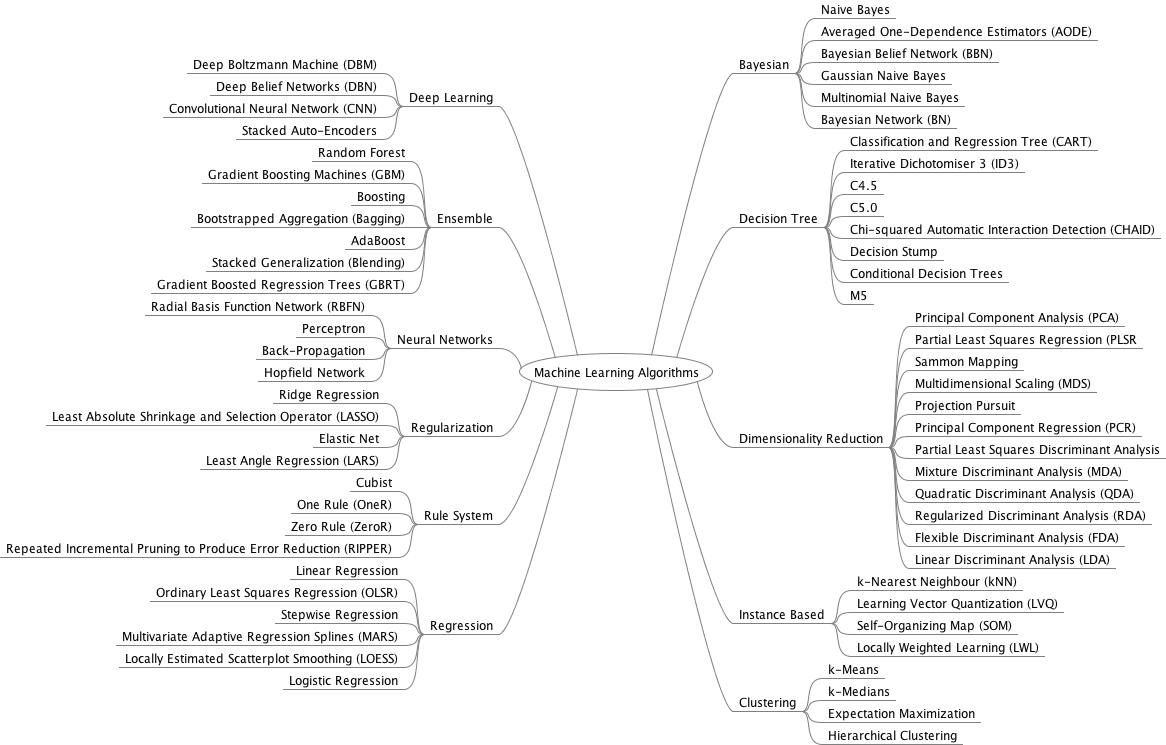
\includegraphics[width=\linewidth]{img/machinelearningalgorithms.png}
	\caption{Mapa mental dos algoritmos de \emph{Machine Learning} organizados por área e sub-área.}
	\label{fig:ml_algorithms}
\end{sidewaysfigure}

Quanto ao tipo de aprendizado, as tarefas de ML podem ser agrupadas em três tipos diferentes, a depender da presença e do tipo de resposta dada ao algoritmo quanto ao desempenho de suas saídas. No \emph{aprendizado supervisionado}, o algoritmo deve aprender a inferir valores a partir de atributos preditores e do respectivo atributo alvo fornecido como exemplo, ou seja, de cenários em que se têm seus valores de saída conhecidos. Os modelos mais comumente utilizados neste tipo de aprendizado são as máquinas de vetores de suporte, redes neurais artificiais \emph{feed-forward}, regressão linear e logística, etc. Já no \emph{aprendizado não-supervisionado}, o algoritmo deve inferir padrões e estruturas a partir de dados não rotulados, buscando alguma estrutura interna que caracterize os dados. Exemplos de modelos aplicáveis a este cenário são os algoritmos \emph{k-means} e \emph{k-medoids}.  Por fim, no \emph{aprendizado por reforço} o algoritmo não recebe dados nem tampouco rótulos, e deve aprender a partir das recompensas positivas ou negativas dadas por ações que modifiquem o ambiente de maneira satisfatória ou não \cite{flach2012machine}.

Quanto ao tipo de saída desejada, os problemas que podem ser endereçados segundo ML são de classificação, regressão, transcrição, tradução automática, detecção de anomalia, síntese e amostragem. No caso do aprendizado supervisionado, em particular, as principais tarefas realizadas são de classificação e regressão \cite{flach2012machine}.

Um algoritmo proposto a uma tarefa de classificação deve especificar cada entrada $x$ como pertencente a uma dentre $k$ categoritas pré-determinadas, produzindo uma saída $y=f(x)$ tal que a função $f$ é definida como $f: \mathds{R}^n \rightarrow \{1, \ldots, k\}$, ou seja, $f$ mapeia sequências de números reais  $x$ de dimensão $n$ para um valor inteiro $y$ dentre $k$ possibilidades \cite{goodfellow2016deep}. Dentre as tarefas de classificação estão, por exemplo, o reconhecimento de objetos em uma imagem, determinar se um indivíduo será ou não vítima de determinada doença, se sobreviverá ou não a determinado acidente, etc.

Numa tarefa de regressão, por sua vez, objetiva-se aprender uma função de valor real a partir de uma entrada \cite{flach2012machine}. Assim, a saída $y=f(x)$ é dada pela função $f: \mathds{R}^n \rightarrow \mathds{R}$, ou seja, $f$ mapeia uma entrada multidimensional $x$ para um valor $y$ real \cite{goodfellow2016deep}. Algumas tarefas de regressão envolvem a previsão de preços de um mercado de ações, a determinação do risco do seguro para um carro, do volume diário de precipitação em determinada cidade, etc.

Os modelos de ML são organizados em dois grandes grupos, dos tipos paramétricos ou não paramétricos. Segundo Russel e Norvig, um modelo de aprendizado que resume dados utilizando um conjunto de parâmetros de tamanho definidos independente do número de exemplos de treinamento é chamado de \emph{modelo paramétrico}. Dentre os modelos paramétricos está a regressão logística. Já um \emph{modelo não-paramétrico}, por sua vez, é aquele que não pode ser caracterizado por um conjunto limitado de parâmetros. Alguns exemplos de modelos não-paramétricos são máquinas de vetores de suporte, redes neurais artificiais, $k$ vizinhos mais próximos e árvores de decisão CART e C4.5 \cite{russell2016artificial}.

Dentre os modelos não paramétricos, as redes neurais artificiais têm demonstrado resultados satisfatórios em tarefas de classificação e regressão quando aplicadas em diversas áreas. Em especial, aplicações de \emph{Deep Learning} no reconhecimento de objetos e no processamento de linguagem natural, por exemplo, têm trazido ainda mais atenção a este modelo. Diante desta importância e da utilização no contexto deste trabalho, estes conceitos serão abordados com mais profundidade nas seções a seguir.


\subsection{Redes Neurais Artificiais} \label{sec:rnas}
%!TEX root = ../../novoIndex.tex

%conceito, inspiração biológica
As \emph{Redes Neurais Artificiais} (RNAs) são um modelo de computação caracterizado por sistemas que, em algum nível, lembram a estrutura do cérebro humano. São sistemas paralelos e distribuídos, compostos por unidades de processamento simples, os \emph{neurônios artificiais}, que calculam funções matemáticas, normalmente não-lineares. Estes neurônios são dispostos em uma ou mais camadas e interligados por um grande número de conexões normalmente unidirecionais e comumente associadas a pesos, que armazenam o conhecimento representado no modelo e ponderam a entrada recebida por cada neurônio da rede. Os principais atrativos das RNAs envolvem a capacidade de capturar tendências a partir de um conjunto de exemplos e dar respostas coerentes para dados não-conhecidos, ou seja, de generalizar a informação aprendida \cite{Teresa:Livro}.

\begin{figure}[hb!]
	\caption{Redes neurais biológicas.}
	\begin{subfigure}[hb]{0.5\linewidth}
		\caption{Neurônio biológico e seus componentes. Fonte: \protect\cite{neuronio_biologico}}
		\label{fig:neuronio_biologico}
		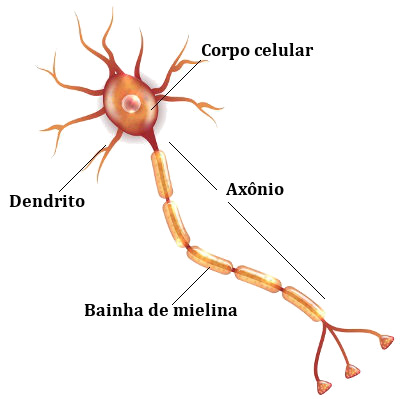
\includegraphics[width=0.7\linewidth]{img/neuronio}
	\end{subfigure}
	\begin{subfigure}[hb]{0.5\linewidth}
		\caption{Sinapse entre neurônios. Fonte: \protect\cite{sinapse}}
		\label{fig:redeneuralbiologica}
		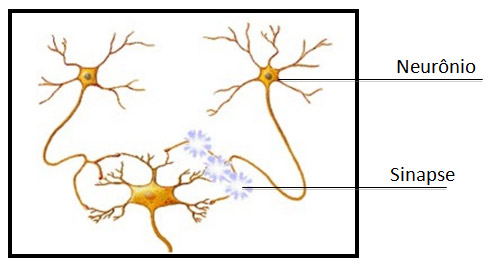
\includegraphics[width=\linewidth]{./img/redeneuralbiologica.jpg}
	\end{subfigure}%
\end{figure}

A motivação para a criação deste modelo vem do funcionamento do cérebro biológico, que é formado por neurônios interligados e que se comunicam entre si de modo contínuo e paralelo através de impulsos nervosos. Esta complexa rede neural biológica é capaz de reconhecer padrões e relacioná-los, produzir emoções, pensamentos, percepcção e cognição. Cada neurônio biológico é composto de um corpo, dendritos e um axônio, como ilustrado na Figura \ref{fig:neuronio_biologico}. Os dendritos são responsáveis pela recepção de impulsos nervosos vindos de outros neurônios; o corpo combina os sinais recebidos pelos dendritos e caso o resultado ultrapasse determinado limiar de excitação do neurônio, são gerados novos impulsos nervosos, que são transmitidos pelo axônio até os dendritos dos neurônios seguintes. Esta conexão unilateral entre neurônios biológicos, denominada sinapse, encontra-se ilustrada na Figura \ref{fig:redeneuralbiologica}.

Com base no modelo biológico, McCulloch e Pitts propuseram em \cite{mcculloch1943logical} um neurônio artificial. Como mostrado na Figura \ref{fig:neuronio}, o modelo de McCulloch e Pitts de neurônio artificial contém $n$ terminais de entrada, denotados por $x = x_1, \ldots, x_n$, e um terminal de saída $y$. Esta organização faz uma alusão aos dendritos, corpo celular e axônio de um neurônio biológico.

\begin{figure}[!ht]
	\centering
	\caption{Representação de um neurônio artificial. Fonte: \cite{neuronio:perceptron}}
	\label{fig:neuronio}
	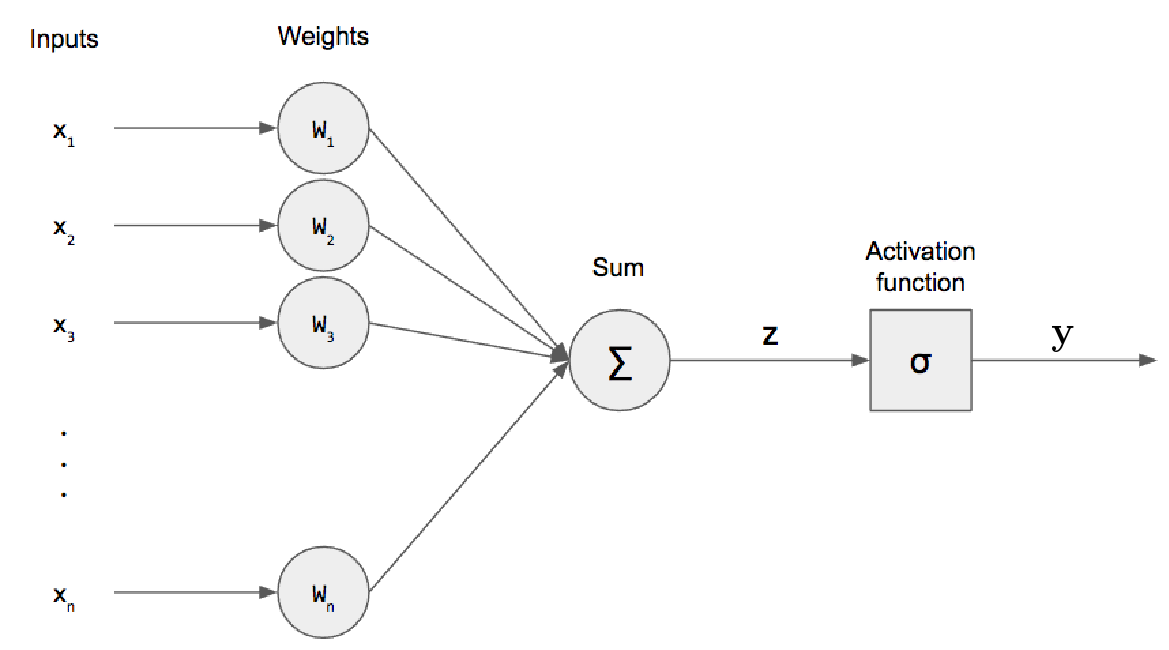
\includegraphics[width=0.7\textwidth]{img/perceptron.png}
\end{figure}
A saída $y$ é o resultado do mapeamento da função de ativação $\sigma$, conforme expresso na Equação \ref{eq:funcao_neuronio}, aplicada à soma ponderada do vetor de entrada $x$ pelo conjunto de pesos $w = w_1, \ldots, w_n$. No caso de um neurônio mais simples, como o de McCulloch e Pitts, a ativação do neurônio é obtida através da aplicação de uma função degrau deslocada, a depender da comparação da entrada com um limiar de ativação $\theta$, conforme Equação \ref{eq:ativacao_limiar} \cite{mcculloch1943logical}.
\begin{eqnarray}
	y &=& \sigma\left( z\right),\label{eq:funcao_neuronio}\\
	z &=& \sum_{i=1}^n x_i w_i\\
	\sigma(z) &=& \begin{cases}
		1, & \text{se } z \geq \theta\label{eq:ativacao_limiar}\\
		0, & \text{caso contrário.}
	\end{cases}
\end{eqnarray}
Considerando desenvolvimentos posteriores, sabe-se atualmente que a escolha da função de ativação $\sigma$ das camadas ocultas e da camada de saída deve considerar funções contínuas e deriváveis \cite{hornik1991approximation}, em que comumente são optadas pelas funções apresentadas na Tabela  \ref{tab:ativacoes}.

 %!TEX root = ../sbc-template.tex

\begin{table}[ht]
	\scalefont{0.8}
	\centering
	\caption{Funçoes de ativação mais populares. ---melhorar legenda}
	\label{tab:ativacoes}
	\begin{tabular}{l l p{6.5cm} l}
		\toprule
		Nome 			 		& Gráfico & Equação & Intervalo\\
		\midrule
		Identidade ou Linear		&
		 	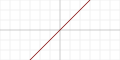
\includegraphics[width=0.1\textwidth]{img/identidade.png}
			&
			$
				\begin{aligned}
					g(z) = z
				\end{aligned}
			$
			& $(-\infty, + \infty) $\\
		\hline
		Tangente Hiperbólica		&
			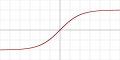
\includegraphics[width=0.1\textwidth]{img/tanh.png}
			&
			$
				\begin{aligned}
					g(z) = tanh(z) =\frac{(e^z - e^{-z})}{(e^z + e^{-z})}
				\end{aligned}
			$
			 & $(-1,1)$\\
		\hline
		Sigmoide ou Logística		&
			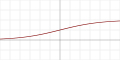
\includegraphics[width=0.1\textwidth]{img/sigmoid.png}
			&
			$
				\begin{aligned}
					g(z) = \sigma(z) = \frac{1}{1+e^{-x}}
				\end{aligned}
			$
			& $ (0,1) $\\
		\hline
		Unidade Linear Retificada	&
			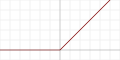
\includegraphics[width=0.1\textwidth]{img/relu.png}
			&
			$
				\begin{aligned}
					g(z) = max(0,z)
				\end{aligned}
			$
			& $ [0, \infty) $\\
		\hline
		Softmax					&
			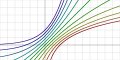
\includegraphics[width=0.1\textwidth]{img/softmax.png}
			&
			$
				\begin{aligned}
					g(\alpha, z) =
						\begin{cases}
							-\frac{ln(1-\alpha(z+\alpha))}{\alpha}, & \text{se } \alpha < 0\\
							z, & \text{se } \alpha = 0 \\
							\frac{e^{\alpha z} -1}{\alpha} + \alpha, & \text{se } \alpha > 0
						\end{cases}
				\end{aligned}
			$
			& $(-\infty, \infty)$\\
		\bottomrule
	\end{tabular}
\end{table}


Em 1958, Frank Rosenblatt desenvolveu o neurônio \emph{Perceptron} \cite{rosenblatt1958perceptron}, que mais tarde seria empregado como a unidade de processamento das RNA e de outros modelos de ML, a exemplo das máquinas de vetores de suporte. O Perceptron de Rosenblatt agregou ao neurônio de McCulloch e Pitts conceitos cruciais para a caracterização das RNAs como são conhecidas hoje, como a não obrigatoriedade de igualdade dos pesos e limiares de ativação, a possibilidade de os pesos serem positivos ou negativos, a diversidade de funções de ativação, entre outros. Além desta caracterização, uma contribuição relevante deste trabalho contempla a proposição de um algoritmo de aprendizado que permite a adaptação dos pesos de uma RNA através da otimização do desempenho da rede. Isto atribuiu ao modelo Perceptron a capacidade de aprender tarefas que contenham dados linearmente separáveis \cite{Teresa:Livro}.

Na ocasião de sua proposição, o modelo Perceptron apresentava algumas limitações, atribuídas principalmente à sua linearidade e simplicidade, características que possibilitam resolver apenas problemas linearmente separáveis \cite{Teresa:Livro}. Com o objetivo de tornar as RNAs aplicáveis em uma gama maior de problemas, os esforços de pesquisadores da área foram concentrados em aumentar e diversificar as técnicas aplicáveis a este modelo. Atualmente, as RNAs podem apresentar diversos tipos de arquitetura, ao variar-se parâmetros como o número de camadas, quantidade de neurônios em cada camada, os tipos de conexões entre neurônios e topologia de rede. Alguns exemplos de arquiteturas podem ser encontrados na Figura \ref{fig:popular_archs}.

\begin{figure}[!ht]
	\caption{Arquiteturas populares de RNAs. Fonte: \cite{rnas_tipos}}
	\label{fig:popular_archs}

	\begin{subfigure}[h]{0.15\linewidth}
		\caption{Perceptron de Camada Única}
		\label{fig:slp}
		\centering
		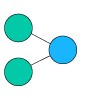
\includegraphics[width=0.6\linewidth]{img/pop_arch/single_layer_perceptron.jpg}
	\end{subfigure}
	\hspace{0.1cm}
	\begin{subfigure}[h]{0.15\linewidth}
		\caption{Radial Basis Network -- RBN}
		\label{fig:rbm}
		\centering
		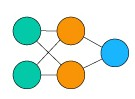
\includegraphics[width=0.9\linewidth]{img/pop_arch/radial_basis_network.jpg}
	\end{subfigure}
	\hspace{0.1cm}
	\begin{subfigure}[h]{0.3\linewidth}
		\caption{Multi Layer Perceptron -- MLP}
		\label{fig:mlp}
		\centering
		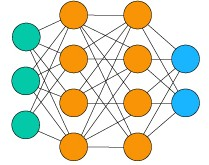
\includegraphics[width=0.75\linewidth]{img/pop_arch/mlp.jpg}
	\end{subfigure}
	\hspace{0.1cm}
	\begin{subfigure}[h]{0.3\linewidth}
		\centering
		\caption{Recurrent Neural Network -- RNN}
		\label{fig:rnn}
		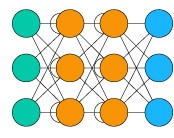
\includegraphics[width=0.6\linewidth]{img/pop_arch/rnn.jpg}
	\end{subfigure}\\

	\begin{subfigure}[h]{0.3\linewidth}
		\centering
		\caption{Long Short-Time Memory RNNs}
		\label{fig:lstm}
		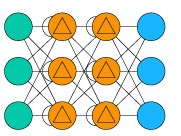
\includegraphics[width=0.6\linewidth]{img/pop_arch/lstm.jpg}
	\end{subfigure}
	\hspace{0.5cm}
	\begin{subfigure}[h]{0.3\linewidth}
		\centering
		\caption{Hopfield Network}
		\label{fig:hopfield}
		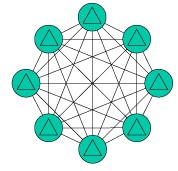
\includegraphics[width=0.6\linewidth]{img/pop_arch/hopfield.jpg}
	\end{subfigure}
	\hspace{0.5cm}
	\begin{subfigure}[h]{0.3\linewidth}
		\centering
		\caption{Boltzmann Machine}
		\label{fig:boltzmann}
		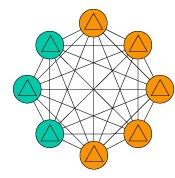
\includegraphics[width=0.6\linewidth]{img/pop_arch/boltzmann.jpg}
	\end{subfigure}
\end{figure}

\begin{table}[H]
	\centering
	\caption{Legenda das unidades presentes nas redes neurais da Figura \ref{fig:popular_archs}.}
	\label{tab:legenda_unidades}
		\begin{tabular}{l l}
			\toprule
			Imagem 			 		& Unidade\\
			\midrule
			\Centerstack{
\includegraphics[width=0.03\textwidth]{img/pop_arch/entrada.jpg}} & Entrada \\
			\hline
			\Centerstack{
\includegraphics[width=0.03\textwidth]{img/pop_arch/saida.jpg}} & Saída \\
			\hline
			\Centerstack{
\includegraphics[width=0.03\textwidth]{img/pop_arch/oculta.jpg}} & Oculta \\
			\hline
			\Centerstack{
\includegraphics[width=0.05\textwidth]{img/pop_arch/feedback_memoria.jpg}} & Feedback com memória \\
			\hline
			\Centerstack{
\includegraphics[width=0.05\textwidth]{img/pop_arch/backfeed.jpg}} & Entrada retroalimentada \\
			\hline
			\Centerstack{
\includegraphics[width=0.05\textwidth]{img/pop_arch/probabilistica.jpg}} & Oculta probabilística \\
			\bottomrule
		\end{tabular}
\end{table}


% Desnecessário
%No que tange à conectividade, uma RNA pode ser classificada como parcialmente ou totalmente conectada. O primeiro caso ocorre quando apenas alguns dos neurônios da camada anterior estão conectados aos da camada posterior. A RNA é dita totalmente conectada se todos os neurônios da camada anterior estão conectados aos da camada posterior.

Quanto aos tipos de conexão possíveis entre os neurônios, tem-se que as RNAs podem ser do tipo \emph{feedforward} ou recorrente. As RNAs \emph{feedforward}, como a exemplificada na Figura \ref{fig:feedforward}, são comumente associadas a um grafo acíclico em que as saídas de uma camada servem de entrada à camada seguinte, e assim sucessivamente, até que seja produzida uma saída da rede. As RNAs recorrentes, tais como a rede exemplificada na Figura \ref{fig:recorrente}, contém conexões entre neurônios de modo a formar um grafo direcionado cíclico, o que permite que o modelo capture sequências de comportamentos organizados em séries temporais.

\begin{figure}[h!]
	\caption{Exemplos de RNA com diferentes tipos de conexões entre neurônios \cite{rna:feedback}.}
	\label{fig:rna_conectividade}
	\begin{subfigure}[h]{0.35\linewidth}
		\caption{Exemplo de RNA \emph{feedforward}.}
		\label{fig:feedforward}
		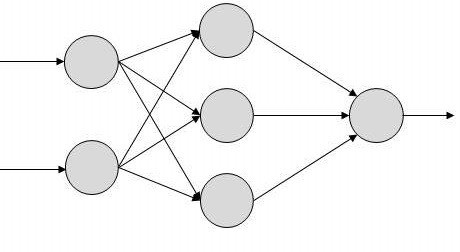
\includegraphics[width=\linewidth]{img/feedforward.jpg}
	\end{subfigure}
	\hfill
	\begin{subfigure}[h]{0.35\linewidth}
		\caption{Exemplo de RNA recorrente.}
		\label{fig:recorrente}
		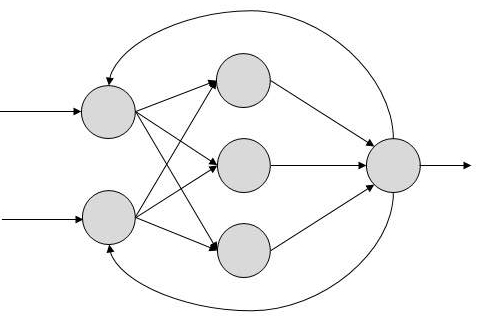
\includegraphics[width=\linewidth]{img/recorrente2}
	\end{subfigure}%
\end{figure}

Um dos parâmetros relacionados à arquitetura de uma RNA é a quantidade de camadas ocultas. Pode-se ter redes de camada única, compostas por um neurônio que conecta todos os parâmetros de entrada às saídas do modelo, a exemplo das redes Perceptron. Há também as redes de múltiplas camadas, que consistem de mais de um neurônio entre entrada e saída da rede, como retratado na Figura \ref{fig:mlp}. Redes com múltiplas camadas, as chamadas Redes Neurais \emph{Feedforward Multilayer Perceptron} (MLP), são capazes de aproximar diversas funções. Quando a Equação \ref{eq:funcao_neuronio} é aplicada a uma camada oculta $c$, de modo que a entrada da função nesta camada seja a saída da camada anterior $c-1$, o resultado $a^{c}$ é construído como mostrado na Equação \ref{eq:funcao_neuronio_camadas} e chamado de mapa de características ou \emph{feature map}. Para uma RNA com profundidade $C$, a saída prevista $\hat{y}$
é dada pelo mapa de característas $a^C$ \cite{hornik1991approximation,Teresa:Livro}.

\begin{gather}\label{eq:funcao_neuronio_camadas}
	z^c = \sum_{i=1}^n a_i^{c-1} w_i^c + b_i^c\\
	a^c = \sigma(z^c)
\end{gather}

Segundo o Teorema da Aproximação Universal definido por Hornik em 1991, se a ativação de uma rede neural MLP for uma função limitada e não-constante, então dada uma entrada $x$, a rede é capaz de aproximar qualquer função contínua, provida uma quantidade adequada de camadas ocultas. Esta característica atribui às redes neurais artificias o potencial de se tornarem máquinas de aprendizado universal \cite{hornik1991approximation}.

\begin{figure}[ht]
	\centering
	\caption{Rede Neural MLP com duas camadas ocultas.}
	\label{fig:mlp}
	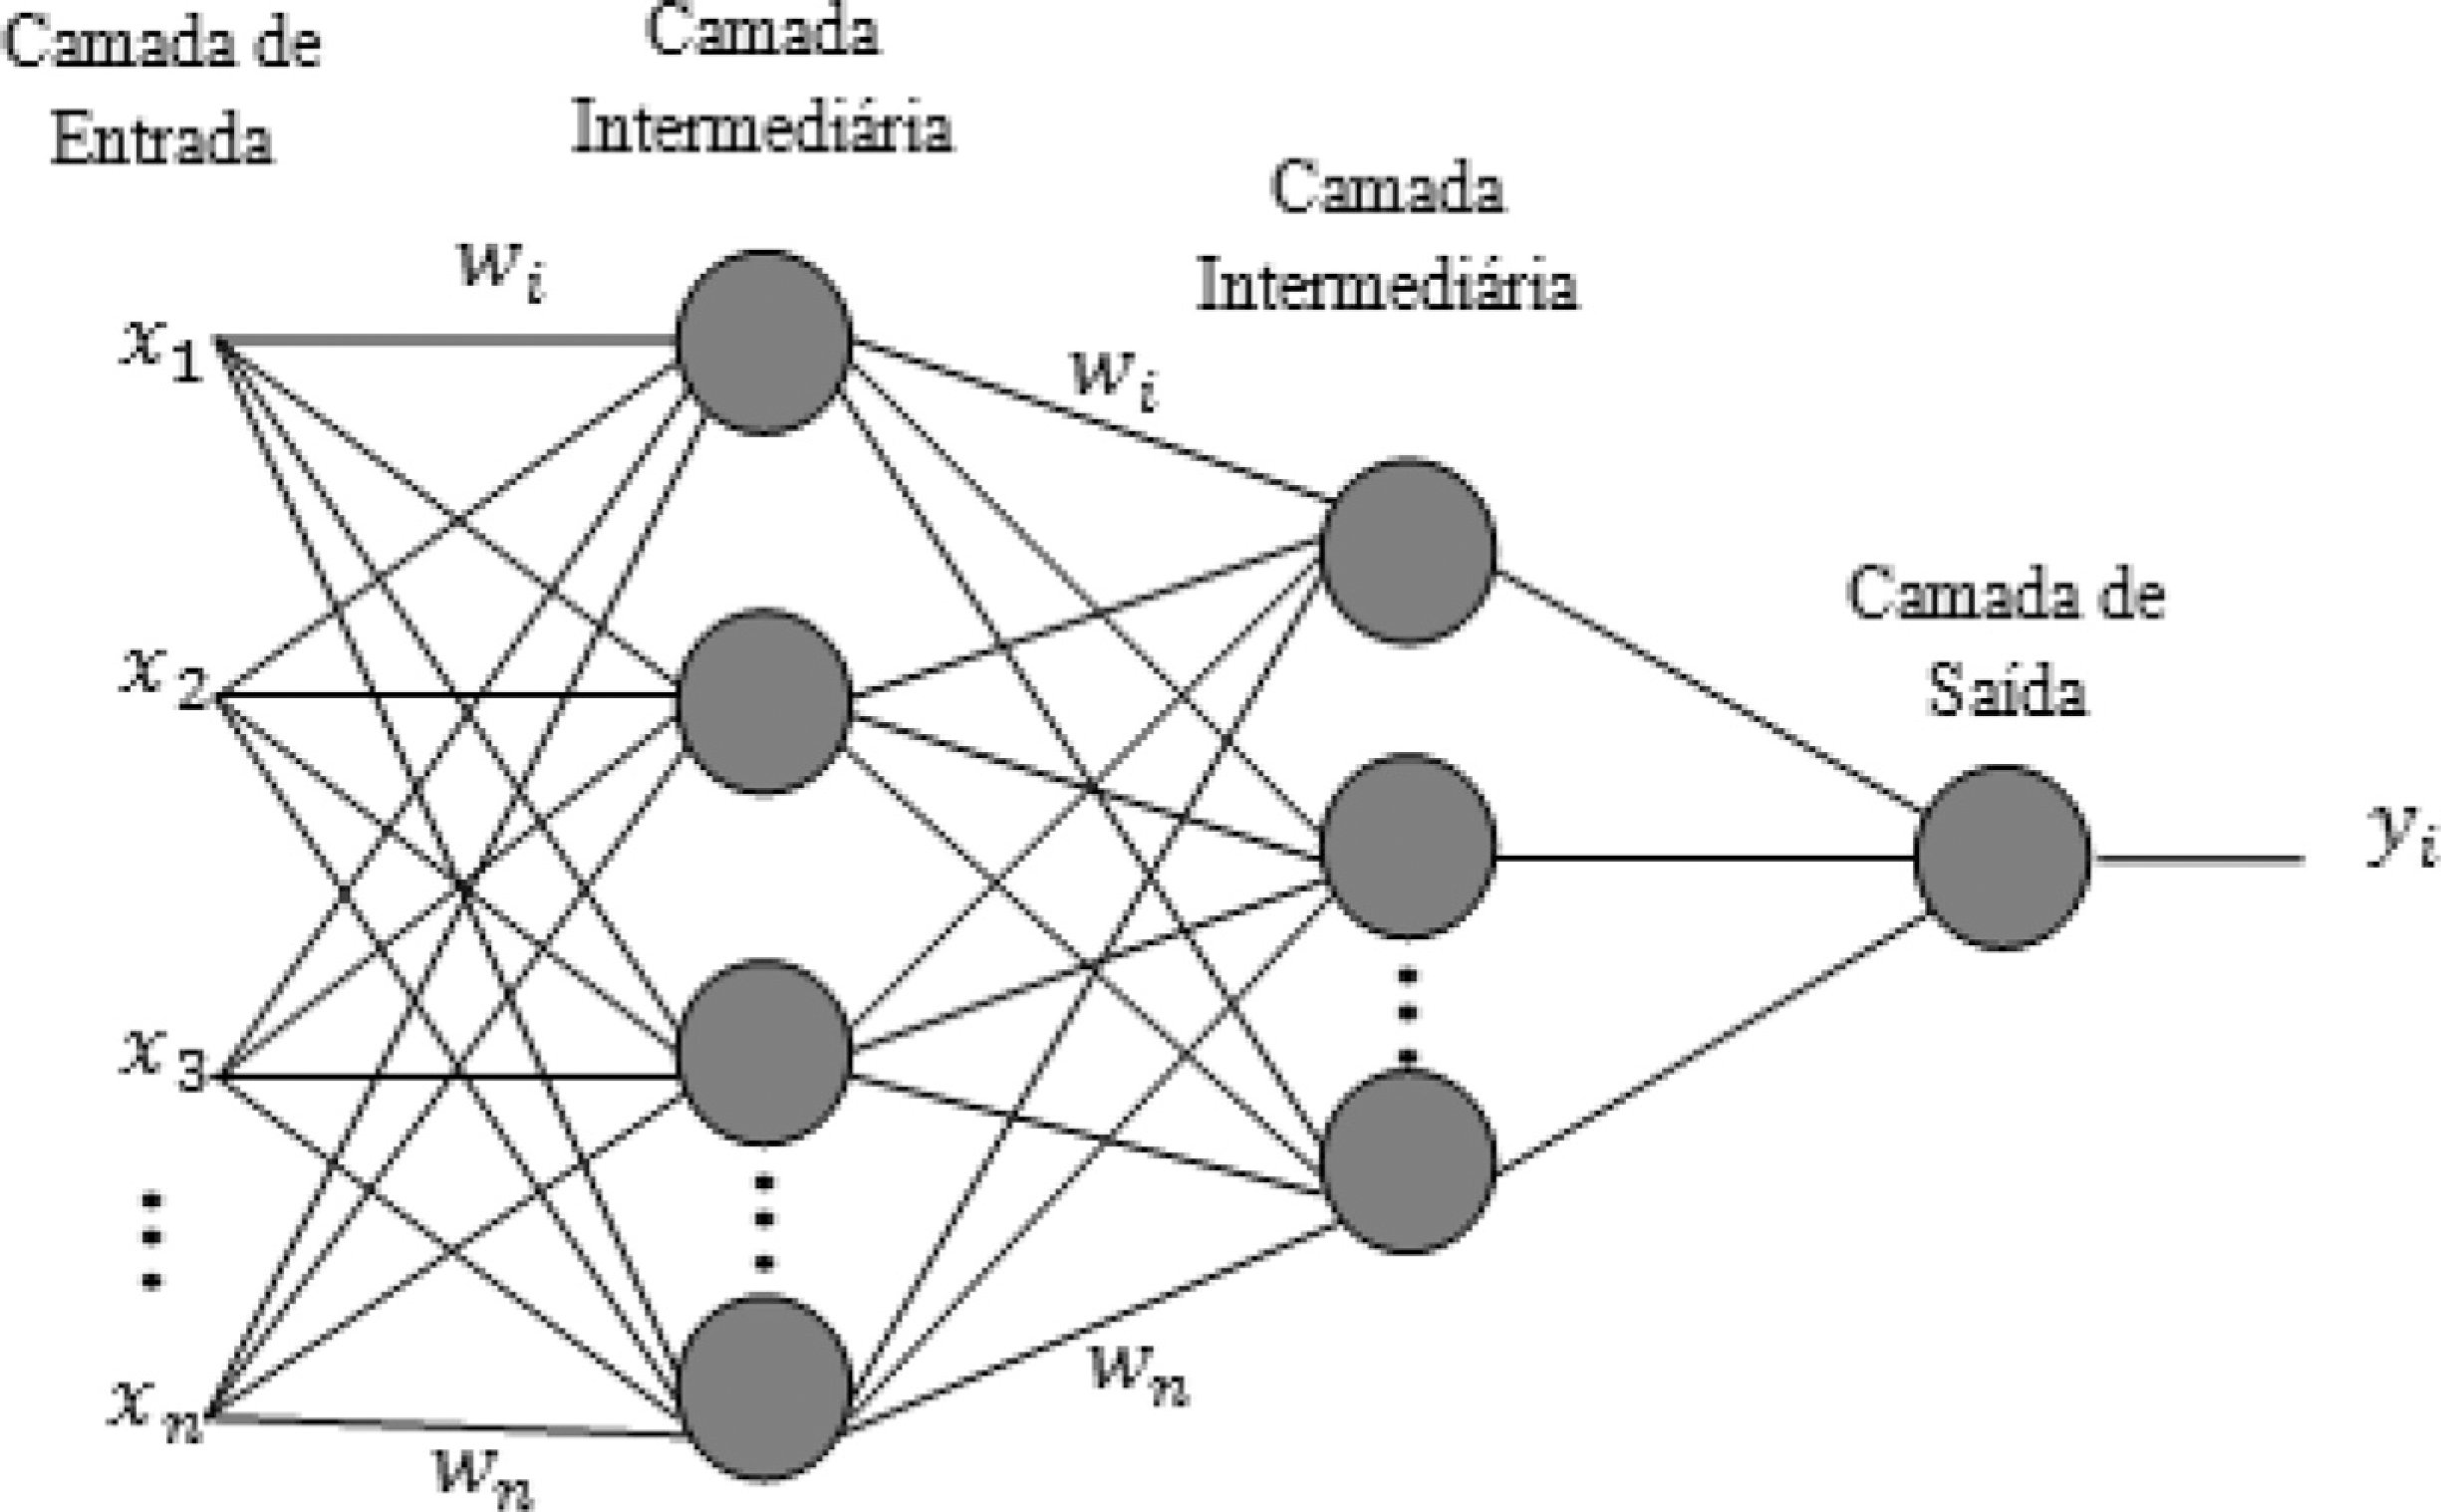
\includegraphics[width=0.6\textwidth]{img/mlprna.jpg}
\end{figure}

O objetivo das RNAs é aproximar funções que mapeiem entradas $x$ às suas respectivas saídas $y$. Para atingir este objetivo, é necessário minimizar a disparidade entre as saídas previstas $\hat{y}$ e as saídas desejadas $y$ através da atualização dos pesos $w$ e do \emph{bias} $b$ dos neurônios das camadas. A função que calcula tal disparidade é chamada \emph{função custo}, dada por $J$ e tida como a soma das funções de perda, $L(\hat{y}_i, y_i)$, entre cada saída esperada $y_i$ e obtida pela RNA $\hat{y}_i$, que é acumulada à medida que o modelo é apresentado a $m$ exemplos do evento que se deseja aprender. A função custo está representada na Equação \ref{eq:custo}, e a perda pode ser calculada de diversas maneiras, a depender do tipo de tarefa de aprendizado, função de ativação e algoritmo de otimização escolhidos.

\begin{equation}\label{eq:custo}
J = \frac{1}{m} \sum_{i=1}^{m} L(\hat{y}_{i}, y_{i}).
\end{equation}

No contexto de maximizar as previsões corretas de uma RNA, deve-se atualizar gradualmente os pesos e \emph{bias} do modelo de maneira a encontrar uma função que melhor represente o comportamento do fenômeno apresentado através dos dados, de maneira a minimizar a função custo para que haja a otimização do desempenho da RNA. Este procedimento é descrito pelo algoritmo de \emph{back-propagation}, que consiste em duas fases que se alternam: a fase \emph{forward} e a fase \emph{backwards} \cite{haykin2009neural}.

A fase \emph{forward}, também chamada \emph{forward propagation}, consiste na inferência das saídas da rede perante um conjunto de $m$ entradas, fornecidas à rede uma de cada vez. Neste processo, dada uma entrada $x_i$, a informação flui para frente  pela rede, isto é, as informações iniciais que são propagadas até as camadas ocultas, e de lá até que a saída $\hat{y}_i$ seja produzida. Ao final de uma fase \emph{forward}, a função custo $J$ é calculada. Modificações presentes na literatura também consideram algumas execuções da fase \emph{forward} para obtenção do custo médio nestas iterações. A representação da sequência de passos realizados nesta fase \emph{forward} está detalhada no Algoritmo \ref{alg:forward} \cite{haykin2009neural, goodfellow2016deep}.

\begin{algorithm}
	\caption{Fase \emph{forward}}\label{alg:forward}
	\Entrada{$i$-ésimo par de exemplos de entrada $x_i$ e saída $y_i$ do conjunto de treinamento}
	\Saida{Perda $L(\hat{y_i}, y_i)$}
	\Inicio{
	A entrada $x_i$ é apresentada à primeira camada da rede, como o primeiro vetor de características $a^0$ \\
	\Para {cada camada c=1,\ldots, C}{
		Calcular a saída da camada $a^c = \sigma^c(z^c)$, $z^c = w^c \times a^{c-1}$\\
	}
	Tomar como valor de saída do modelo a saída da última camada $\hat{y} = h^C$\\
	Calcular a perda $L(\hat{y_i}, y_i)$.
	}
\end{algorithm}

A fase \emph{backwards} é responsável por permitir que a informação referente à diferença entre os valores de saída obtidos $\hat{y}$ e os esperados $y$ calculada através da função custo na fase \emph{forward} flua para trás. Isto ocorre por meio da atualização dos pesos dos neurônios, a começar por aqueles localizados na camada de saída, passando pelas camadas ocultas, até atingir a camada de entrada. Ao percorrer este caminho contrário, para cada camada é calculado o gradiente $\delta$ da perda $L$ em função dos pesos e \emph{bias}, dado pela fórmula mostrada na Equação \ref{eq:gradiente}.

\begin{gather}\label{eq:gradiente}
	\delta_w = \nabla_{w} J = \left[
							\frac{\partial J}{\partial w_1}, \frac{\partial J}{\partial w_2}, \ldots, \frac{\partial J}{\partial w_n}
						\right]^T\\
	\delta_b = \nabla_{b} J = \left[
							\frac{\partial J}{\partial b_1}, \frac{\partial J}{\partial b_2}, \ldots, \frac{\partial J}{\partial b_n}
						\right]^T
\end{gather}

No contexto do cálculo, o gradiente indica o sentido e a direção para as quais se devem mover os valores dos pesos e \emph{bias} das camadas de maneira a se obter o maior incremento possível de perda. Considerando que o objetivo consiste na minimização \emph{gradual} dos parâmetros da rede na iteração $t+1$, o ajuste dos pesos e \emph{bias} dos neurônios na iteração $t$ é comumente realizado por meio do método gradiente descendente indicado na Equação \ref{eq:gradiente_descendente}, no qual o valor do gradiente $\delta$ é multiplicado por uma taxa de aprendizado $\eta$ e então subtraído dos valores de $w$ e $b$ \cite{haykin2009neural, goodfellow2016deep}.

\begin{gather}\label{eq:gradiente_descendente}
	w^c(t+1) = w(t) - \eta \nabla_{w^c} \\
	b^c(t+1) = b(t) - \eta \nabla_{b^c}
\end{gather}

A fase \emph{backwards}, denotada no Algoritmo \ref{alg:backpropagation}, lança mão de sequências de operações de regras da cadeia para calcular os gradientes. Inicialmente, o gradiente $\delta$ da função de ativação $\sigma$ da camada $l$ é obtido ao realizar o produto interno do gradiente calculado sob a função de custo da RNA pela derivada da função de saída $\sigma^c$. Esta combinação de derivações encadeadas é altamente eficiente, o que faz com que o o custo operacional da computação do gradiente seja $O(m)$, sendo $m$ o número de exemplos no conjunto de treinamento. Assim, o custo computacional cresce de maneira proporcional e linear à quantidade de exemplos presentes no conjunto de treinamento \cite{haykin2009neural, goodfellow2016deep}.

\begin{algorithm}
	\caption{Fase \emph{backwards}.}\label{alg:backpropagation}
	\Entrada{Custo $J$}
	\Saida{Gradientes dos parâmetros da RNA MLP atualizados}
	\Inicio{
		Calcular gradiente do custo, ou seja, da perda da camada de saída $\delta = \nabla_y J = \nabla_y L(\hat{y_i},y_i)$\\
		\Para {cada camada c=C,\ldots, 1}{
			Calcular o gradiente da camada $c$, dado por $\delta^c = \delta^{c-1} \cdot \sigma^c(z^c)$\\
			Atualizar variação em $w$, dada por $\nabla_{w^c} = \delta^c  a^{(c-1)}$\\
			Atualizar variação em $b$, dada por $\nabla_{b^c} = \delta^c$
		}
	}
\end{algorithm}

Além dos parâmetros $w$ e $b$, as RNAs MLP têm hiperparâmetros, responsáveis por controlar as mudança ocorridas nos parâmetros. Bengio define hiperparâmetros como variáveis cujos valores devem ser definidos antes que o algoritmo de treinamento se inicie. Alguns hiperparâmetros já discutidos neste texto são a taxa de aprendizado $\eta$, número de camadas ocultas, quantidade de neurônios e tipos de funções de ativação escolhidos para cada camada. O número de vezes que o conjunto de dados é apresentado ao modelo no treinamento, conhecido como número de épocas, também é um hiperparâmetro, assim como a quantidade de exemplos de treinamento apresentados à rede de uma só vez na fase \emph{forward}, chamado de \emph{batch size} \cite{bengio2012practical}.

Sumarizando os conceitos apresentados, o algoritmo para treinamento supervisionado de uma RNA MLP se dá como mostrado no Algoritmo \ref{alg:treinamento}.

\begin{algorithm}[h!]
	\caption{Algoritmo de treinamento de uma RNA  \cite{Teresa:Livro}.}\label{alg:treinamento}
	\Entrada{Conjuntos de exemplos e respectivos rótulos $(X,Y)$, rede neural a ser treinada, número de épocas $e$, taxa de aprendizado $\eta$ e \emph{batch size} $b$.}
	\Saida{Rede neural treinada.}
	\Inicio{
		Inicialização dos vetores de pesos $w$ e \emph{bias} $b$\\
		\Para {cada \emph{batch} = 1,\ldots, b do conjunto de dados}{
			Fase \emph{forward}: Calcular previsões $\hat{y}$ e custos $J$.\\
			Fase \emph{backwards}: Calcular gradientes dos pesos $\nabla_{w^c}$ e \emph{bias} $\nabla_{b^c}$\\
			Atualizar valores dos pesos e \emph{bias} a partir do gradiente descendente.
		}
	}
\end{algorithm}

Ao lidar com técnicas que visam acelerar ou potencializar o processo de aprendizado, o número de hiperparâmetros aumenta. Alguns exemplos destas técnicas incluem os algoritmos que realizam a otimização do gradiente descendente através da regularização dos pesos, como a Estimação Adaptativa do Momento, ou \emph{Adam} e o algoritmo de otimização da família dos métodos quase Newtonianos \emph{L-BFGS}. Outros hábitos comuns incluem a adoção de métodos de inicialização dos pesos que evitem o gradiente de convergir para pontos de sela, e de uma taxa de aprendizado que diminui conforme o número de épocas executadas aumenta para que o gradiente convirja para um ponto mínimo mais rapidamente \cite{goodfellow2016deep}.

As RNAs \emph{feedforward} MLP são amplamente utilizadas em aplicações de diversos domínios. Inicialmente, destacaram-se as aplicações voltadas para o mercado financeiro visando, por exemplo, otimizar estratégias de marketing. Aplicações posteriores consideraram a alocação de assentos em aviões, aprovação de empréstimo, controle de qualidade em processos industriais, dentre outros \cite{widrow1994neural}. O escopo de aplicações deste modelo continua a crescer nos dias atuais, especialmente diante do desenvolvimento de variantes, a exemplo das redes neurais convolucionais, com grande capacidade de detecção de padrões e pouco esforço de pré-processamento. Reconhecimento de caracteres e dígitos  \cite{lenet}, processamento de imagens médicas para reconhecimento de características associadas à doenças cardíacas \cite{oktay2018anatomically}, pulmonares \cite{mingchen2018holistic} e mamárias \cite{dubrovina2018mammography} são alguns exemplos de aplicações de vanguarda destes modelos compreendidos dentro da sub-área de \emph{Deep Learning}, que será caracterizada na seção a seguir.


\subsection{\emph{Deep Learning}}\label{sec:dl}
%!TEX root = ../../novoIndex.tex

\emph{Deep Learning} (DL), também conhecido como Aprendizado Profundo, compreende um conjunto de técnicas de ML que podem ser aplicadas em problemas de aprendizado supervisionado e não-supervisionado. A principal característica dos modelos neste domínio é a capacidade de representar e reconhecer características sucessivamente complexas, por meio da adição de níveis ou camadas de operações não-lineares em sua arquiteturas, a exemplo das redes neurais profundas, máquinas de Boltzmann profundas e fórmulas proposicionais. Modelos deste tipo ganharam popularidade ao se mostraram capazes de resolver problemas complexos com um desempenho cada vez maior \cite{bengio2009learning}.

A melhoria do desempenho de modelos de DL é decorrente do aumento recente da quantidade de dados disponíveis sobre temas complexos, aliado ao aumento da disponibilidade de recursos computacionais para executar modelos mais robustos \cite{goodfellow2016deep,deng2014deep}. Alguns dados fornecidos pela IBM reforçam esta afirmação: em $2017$ foram gerados $2,5$ quintilhões de bytes de dados por dia, e $90\%$ do volume total de dados gerados até $2017$ no mundo foi criado somente nos últimos dois anos \cite{ibm2017bigdata}. Estes fatores possibilitaram a implementação de modelos que apresentaram uma melhoria significativa na eficiência de generalização frente a modelos existentes até então, especialmente em virtude da capacidade de organizar a computação como uma composição de várias operações não-lineares (funções de ativação) e uma hierarquia de características re-utilizadas (adição de camadas) \cite{goodfellow2016deep}.

Para exemplificar o efeito da adição de camadas aos modelos de DL, a Figura \ref{fig:compara_redes} mostra uma visão geral do aumento da profundidade das camadas de redes neurais e o desempenho destas em problemas de detecção de objetos em imagens. Nota-se que, à medida que a profundidade aumenta, há uma diminuição no erro. Mais recentemente, isto também tem implicado na redução do número de parâmetros treináveis, por meio da implementação de técnicas de subamostragem \cite{haykin2009neural}. Este panorama reforça a hipótese de que o aumento da profundidade das redes neurais impacta positivamente na captura de características e que estes avanços têm tornado as tarefas mais factíveis, com uma diminuição do esforço computacional associado, em comparação com modelos mais rasos \cite{goodfellow2016deep}.

\begin{figure}[ht]
	\centering
	\caption{Evolução de profunidade, taxa de erro e número de parâmetros das redes neurais profundas com o passar dos anos. Fonte: \cite{mediumcnn}.}
	\label{fig:compara_redes}
	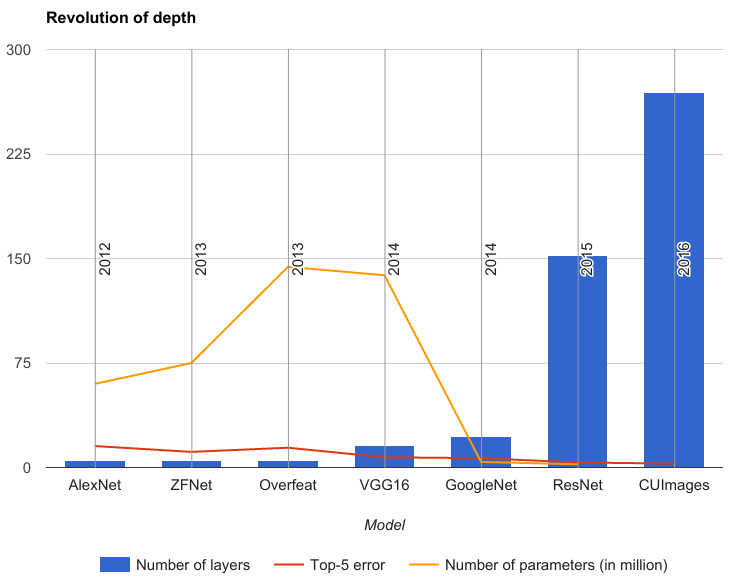
\includegraphics[width=0.8\textwidth]{img/compara_redes.png}
\end{figure}

\subsection{Breve Histórico}

O termo \emph{Deep Learning} (DL) não é recente, foi utilizado pela primeira vez por Dechter, no contexto da descoberta de todas as configurações de conflitos mínimas a fim de resolver um problema de satisfação de restrições \cite{dechter1986learning}. Porém, ganhou força a partir de pesquisas sobre RNAs \emph{feedforward} com muitas camadas ocultas, também conhecidas por redes neurais profundas \cite{deng2014deep}.

Considera-se que o desenvolvimento de DL pode ser dividido em três momentos. No primeiro momento, houve a proposição de modelos lineares simples, compostos apenas por um neurônio, a exemplo dos neurônios de McCulloch e Pitts \cite{mcculloch1943logical} e \emph{Perceptron} de Rosenblatt  \cite{rosenblatt1958perceptron}. No segundo instante, iniciado nos anos 1980, teve-se como eixo central a interconexão entre vários neurônios e a proposição do algoritmo \emph{back-propagation} para ajuste de pesos no treinamento das RNAs \cite{rumelhart1986parallel,rumelhart1986backpropagation}. Com estas contribuições, houve aplicação das RNAs em diversos domínios. Ainda no final deste segundo momento, duas contribuições relevantes foram feitas: os modelos \emph{Long Short-Term Memory} (LSTM) e LeNet. Esta última utiliza o algoritmo de \emph{backpropagation} para treinar uma rede neural convolucional profunda para reconhecer dígitos escritos à mão \cite{lenet}.

A terceira fase tem um marco inicial definido: compreende o ano de $2006$, quando Hinton utilizou o termo \emph{deep belief network} para designar um tipo de modelo de RNA MLP cujo treinamento adota uma estratégia gulosa e orientada a camadas. Cada camada é pré-treinada individualmente como uma máquina de Boltzmann restrita, e o modelo inteiro é então ajustado utilizando técnicas de treinamento supervisionado, incluindo o algoritmo de \emph{backpropagation}. A partir deste marco, outros pesquisadores passaram a investigar a técnica de Hinton e, com o tempo, o termo \emph{deep learning} passou a designar modelos compostos de várias camadas sucessivas de operações não lineares utilizados para o aprendizado de determinada tarefa \cite{hinton2006fast, hinton2007learning, goodfellow2016deep, deng2014deep}.

Na conjectura atual, modelos de DL têm superado significativamente o estado da arte de modelos inteligentes em diversas competições em todo o mundo. A \emph{ImageNet Large Scale Visual Recognition Challenge} (ILSVRC) \cite{ImagenetChall} é uma competição em que equipes de pesquisa avaliam seus algoritmos em um conjunto de dados fornecido, e competem para chegar à melhor acurácia em várias tarefas de reconhecimento visual automático. O conjunto de dados utilizado, denominado ImageNet \cite{Imagenet:main}, consiste de um conjunto de aproximadamente $14$ milhões de imagens de $21$ mil categorias organizadas hierarquicamente, em que cada uma contém algumas centenas de imagens de exemplo. A performance dos modelos submetidos para a competição é chamada taxa de erro top-5, e representa o erro computado quando a classe alvo não se encontra entre as 5 apontadas pelo modelo como as que têm maior probabilidade de estarem na imagem. Em 2011, os melhores resultados de  classificação no ILSVRC tinham por volta de $25\%$ de erro top-5 nas tarefas propostas. Em 2012, o modelo AlexNet, uma rede neural convolucional proposta segundo as ideias de DL, atingiu apenas $16,4\%$ de erro, propondo um ganho até então nunca visto entre duas edições sucessivas da competição \cite{ImagenetChall:2012}.

O gráfico da Figura \ref{fig:compara_redes} sintetiza o histórico da competição ILSVRC, em que a partir do ano de 2012 houve a introdução de modelos baseados em DL. O histograma mostra a diminuição do erro na tarefa de aprendizado proposta e a linha tracejada enfatiza o número de camadas ocultas utilizadas nos modelos vencedores.

\begin{figure}[ht]
	\centering
	\caption{Evolução do erro dos modelos vencedores da competição ILSVRC pela profundidade das redes neurais \cite{dl_ILSVRC, ImagenetChall}}
	\label{fig:compara_redes_ilsvrc}
	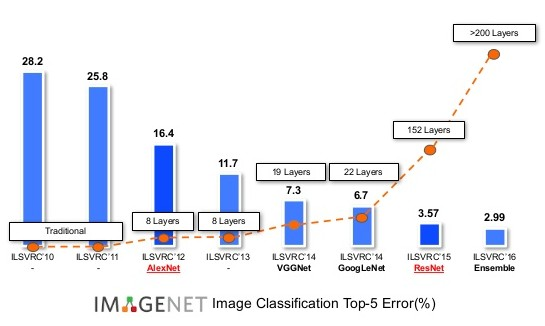
\includegraphics[width=0.8\textwidth]{img/compara_redes_ilsvrc.png}
\end{figure}

Apesar do foco inicial de DL ter sido concentrado no desenvolvimento de técnicas de aprendizado não-supervisionado e na habilidade de modelos profundos de boa generalização a partir de conjuntos de dados pequenos, o cenário atual das pesquisas nesta área consideram o uso de técnicas de aprendizado supervisionado visando o endereçamento de conjuntos de dados massivos e categorizados, e também redes neurais profundas híbridas, que misturem técnicas e conceitos de diferentes origens \cite{deng2014deep,goodfellow2016deep}.

Dentre estes resultados de vanguarda no ILSVRC destacam-se os modelos de DL construídos com redes neurais convolucionais, que têm impulsionado os mais recentes avanços na área de Visão Computacional desde a proposição na literatura da rede LeNet \cite{lenet}. Em particular, desde a proposição e vitória do modelo AlexNet \cite{alexnet} no ano de 2012, as redes neurais convolucionais têm dominado o ranking dos anos seguintes da competição, conforme ilustrado na Figura \ref{fig:compara_redes_ilsvrc} \cite{deng2014deep}. Dada a importância deste tipo de rede neural, os conceitos sobre as mesmas e os modelos canônicos serão apresentados a seguir.


\subsection{Redes Neurais Convolucionais} \label{subsubsec:rnc}
%!TEX root = ../../sbc-template.tex
\emph{Redes Neurais Convolucionais} (CNNs, do inglês \emph{Convolutional Neural Networks}) são uma classe de redes neurais \emph{feedforward} com topologia bem definida e estrutura em grade, com o uso de operações de convolução em pelo menos uma de suas camadas \cite{goodfellow2016deep}. Aplicadas em tarefas de classificação, regressão, localização, detecção e outras, este tipo de modelo se destaca no reconhecimento de padrões em dados de alta dimensionalidade, a exemplo de séries temporais, imagens e vídeos \cite{Khan:Livro}.

A operação de convolução possui um papel central nas CNNs. Esta operação descreve a média ponderada de uma determinada função $x_1(t)$ sob um intervalo fixo de uma variável, enquanto os pesos da média ponderada considerada pertencem à função $x_2(t)$ amostrados em intervalos $a$ \cite{bracewell1986fourier}. Assim, a convolução $s(t)$ de duas funções $x_1(t)$ e $x_2(t)$ é uma função $s: \mathds{Z} \rightarrow \mathds{R}$, denotada $s(t) = x_1(t) * x_2(t)$, e definida conforme Equação \ref{eq:int_convolucao} \cite{lathi2006sinais}:

\begin{equation}\label{eq:int_convolucao}
s(t) = x_1(t) * x_2(t) = \int_{-\infty}^{\infty} x_1(a) x_2(t-a)da.
\end{equation}

No contexto de ML, a função $x_1(t)$ é chamada de \emph{input}, a função $x_2(t)$ é o \emph{kernel}, e a saída $s(t)$ consiste no \emph{feature map}, ou mapa de características. No contexto prático, o \emph{input} normalmente é um vetor multidimensional de dados e o \emph{kernel} é um vetor multidimensional de pesos que devem ser ajustados para aprendizado das CNN. Considerando, por exemplo, uma imagem $I$ de dimensões $(m,n)$ como \emph{input} e a aplicação de um \emph{kernel} $K$, a versão discreta da convolução, passível de implementação computacional e equivalente à Equação \ref{eq:int_convolucao}, é mostrada na Equação \ref{eq:conv_img}:
\begin{equation}
 S(i,j) = I(i,j)*K(i,j) = \sum_{m}\sum_{n}I(m,n)K(i-m,j-n),\label{eq:conv_img}
\end{equation}
em que $S$ é o \emph{feature map} resultante e $(i,j)$ é a posição correspondente nesse mapa. Para otimizar os aspectos de implementação, os valores resultantes da operação de convolução são armazenados apenas nas posições $(i,j)$ explicitamente declaradas \cite{goodfellow2016deep}.

Os \emph{feature maps}, resultantes das operações de convolução, compreendem a noção de filtros, responsáveis por capturarem características relativas à entrada, tais como contornos, linhas, texturas, etc. Quando combinados de maneira sequencial, como proposto pelas CNNs, as características capturadas pelas camadas convolucionais vão se tornando mais complexas à medida que se aumenta a profundidade da rede. Assim, um primeiro \emph{feature map} de uma camada convolucional captura um simples contorno, enquanto um \emph{feature map} em uma camada mais profunda da rede pode capturar uma forma, um rosto ou até um objeto inteiro \cite{Buduma:Livro}. Esta noção é ilustrada na Figura \ref{fig:convolutions}.

\begin{figure}[!h]
	\centering
	\caption{Papel das camadas convolucionais e \emph{feature maps} nas CNNs. Fonte: \cite{Khan:Livro}.}
	\label{fig:convolutions}
	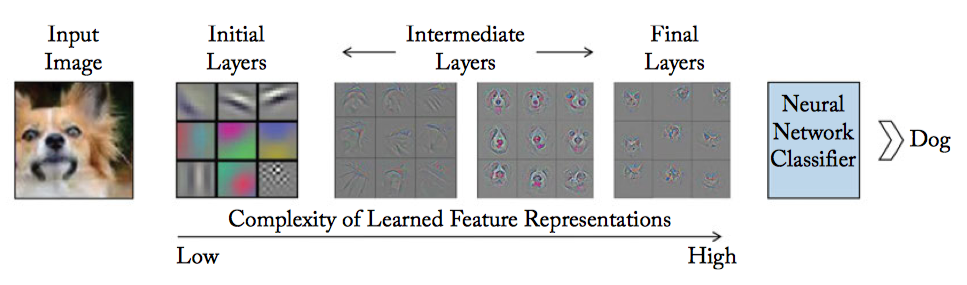
\includegraphics[width=0.8\textwidth]{./img/fundamenta/convolutions}
\end{figure}

As camadas convolucionais, que capturam os \emph{feature maps} e contém os pesos da rede, normalmente são seguidas por funções de ativação como as exemplificadas na Seção \ref{sec:rnas}, mais especificamente na Tabela \ref{tab:ativacoes}. Via de regra, a toda camada convolucional em uma CNN, segue-se uma função de ativação, finalizando em uma operação de \emph{pooling}, como mostra a Figura \ref{fig:cnn_camada}.

\begin{figure}
	\centering
	\caption{Componentes de uma camada de uma rede neural convolucional \cite{goodfellow2016deep}.}
	\label{fig:cnn_camada}
	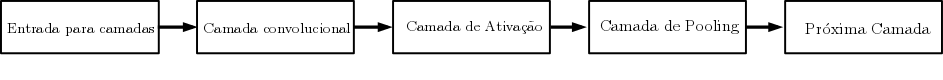
\includegraphics[width=\textwidth]{img/cnn_camada_ipe.png}
\end{figure}

 Uma função de \emph{pooling} substitui a saída da rede em determinada localização por uma síntese estatística das saídas vizinhas. Por exemplo, a operação \emph{max pooling} retorna o valor máximo em uma área retangular, enquanto a \emph{average pooling} retorna a média das saídas de um retângulo. O objetivo desta operação é fazer com que o \emph{feature map} seja invariante a pequenas mudanças na entrada. Esta invariância à pequenas mudanças locais é uma propriedade útil quando o mais importante for a existência da característica e não exatamente a sua posição, o que aumenta a eficiência geral da CNN ao reduzir drasticamente o número de valores a serem passados entre duas camadas quaisquer \cite{goodfellow2016deep}.

 Outros parâmetros, como \emph{padding} e \emph{strides}, são importantes para a captura de características. O parâmetro \emph{padding} consiste em adicionar um número de linhas e colunas em cada lado da entrada de maneira a controlar o tamanho do \emph{feature map} resultante da operação de convolução. Já a distância entre duas janelas da convolução, ou da operação de \emph{pooling}, é medida através do número de \emph{strides}. Ambos parâmetros manipulam as dimensões das saídas das camadas de uma CNN \cite{chollet2017deep}.

Embora se tenha uma noção clara das camadas individuais e de suas respectivas funções, a combinação das mesmas em uma rede neural convolucional não é uma tarefa trivial, podendo resultar em um número arbitrariamente grande de redes com milhares de parâmetros ajustáveis, cujo desempenho acerca de um problema ainda precisará ser aferido. Considerando os esforços computacionais para isto, a maioria das soluções atuais baseadas em DL fazem uso de CNNs canônicas já propostas na literatura, as quais são apresentadas a seguir.


\subsection{Modelos Canônicos de Redes Neurais Convolucionais} \label{subsubsec:modelos_canonicos}
%!TEX root = ../../sbc-template.tex

Os modelos canônicos de CNNs são arquiteturas que trouxeram contribuições importantes, pioneiras na aplicação de técnicas que são comuns ainda hoje no cenário de DL, comumente utilizadas em diversas tarefas de aprendizado \cite{9dlpapers}.

A LeNet é o primeiro modelo de rede neural a aplicar convoluções ao invés das camadas totalmente conectadas convencionais. Foi proposta por LeCun em 1998 e é composta de 7 camadas, sendo uma camada de entrada, duas camadas convolucionais, duas camadas de \emph{pooling}, uma camada totalmente conectada e a camada de saída. A tarefa de aprendizado endereçada por esta rede na ocasião de sua proposição foi o reconhecimento de dígitos manuscritos. Para o treinamento e teste desta rede foi utilizado o conjunto de dados \emph{Modified National Institute of Standards and Technology} (MNIST), composto de 60000 imagens de treinamento e 10000 de teste dos dígitos de 0 a 9 escritos à mão \cite{mnist}. A LeNet foi amplamente utilizada por bancos para o reconhecimento de números escritos à mão em cheques digitalizado em imagens em escala de cinza de tamanho $32 \times 32$ \cite{lenet}. Apesar de pesquisas nesta área continuarem no decorrer dos anos, a quantidade insuficiente de bases de imagens catalogadas e o baixo poder computacional da época fizeram com que as CNNs permanecessem sem grandes destaques até o ano de 2012 \cite{9dlpapers}.

AlexNet foi a primeira CNN ganhadora do desafio ILSVRC, em 2012, ao atingir um erro top-5 igual a $15.4\%$. O segundo melhor modelo daquele ano atingiu um erro de $26.2\%$. Esta rede, treinada para uma tarefa de classificação utilizando imagens de 1000 categorias da ImageNet, é formada por 5 camadas convolucionais com filtros de tamanho $11 \times 11$, intercaladas com camadas de \emph{max-pooling} e \emph{dropout} e $3$ camadas totalmente conectadas. Utilizava a função de ativação \emph{ReLU} ao invés da tradicional tangente hiperbólica. Na ocasião, para obter uma quantidade de exemplos razoável mediante o número de parâmetros ajustáveis, foi realizado um aumento artificial nas imagens de entrada, modificando-as segundo translações, reflexões horizontais e cortes. A AlexNet foi então treinada utilizando duas GPU GTX 580 por 5 a 6 dias, com o algoritmo de \emph{backpropagation} utilizando gradiente descendente estocástico para \emph{batch} e técnicas como \emph{momentum} e \emph{weight decay}. Estas técnicas garantiram à rede um desempenho significativamente melhor que o dos modelos tradicionais que estavam sendo aplicados para a ILSVRC daquele ano \cite{alexnet}.

Uma CNN que com um amplo destaque pela simplicidade e profundidade é a VGG. Apesar de não ter ganhado a ILSVRC 2014, alcançou um erro top-5 de $7.3\%$. Foi concebida na Universidade de Oxford, a VGG-19 contendo 19 camadas que utiliza estritamente filtros de $3 \times 3$ com \emph{stride} e \emph{pad} de 1, juntamente com \emph{max-pooling} de tamanho $2 \times 2$ e \emph{stride} 2. O número de filtros dobra após cada camada de \emph{max-pooling}, o que reforça a idéia de diminuir dimensões espaciais de largura e altura e aumentar a profundidade. A VGG-19 foi treinada em parte da base ImageNet utilizando 4 GPUs Nvidia Titan Black por duas a três semanas \cite{vggnet}.

Uma das primeiras arquiteturas de CNNs que se desviou do caminho normal de simplesmente empilhar camadas convolucionais e de pooling em uma estrutura sequencial foi a GoogLeNet, também chamada de Inception. Dotada de 22 camadas convolucionais, a rede ganhou o ILSVRC 2014 com um erro top-5 de $6.7\%$. Esta performance se deve aos chamados de módulos Inception, compostos de camadas da rede que ocorrem em paralelo. Ao invés de realizar uma operação de convolução ou \emph{max-pooling} de cada vez, várias operações diferentes são realizadas e os mapas de características obtidos são condensados e conectados ao próximo bloco Inception. A Figura \ref{fig:bloco_inception} mostra que há 4 conjuntos de operações a serem realizadas, todas contendo convoluções com filtros $1 \times 1$, podendo haver também a convolução com filtros de tamanho $3 \times 3$, $5 \times 5$, ou uma operação de \emph{max-pooling} de $3\times 3$. A convolução com filtro $1\times 1$ é aplicada para reduzir a dimensionalidade do problema reduzindo a profundidade do mapa de características, além de retirar da entrada informações bem detalhadas em volume. As convoluções que utilizam filtros de $3\times 3$ e $5\times 5$ dão ao modelo a capacidade de extrair informações relevantes em larga escala. A camada de \emph{max-pooling} é aplicada a fim de reduzir a largura e altura do mapa de característas e combater \emph{overfitting}. Na GoogLeNet, as camadas totalmente conectadas são substituídas por \emph{average pooling}, o que economiza um grande número de parâmetros. A rede, que foi treinada em algumas GPUs de alta performance por uma semana, utiliza ReLU como função de ativação e dispõe de 9 módulos Inception com mais de 100 camadas no total. Todas estas técnicas utilizadas para reduzir a dimensionalidade do problema surtiram efeito pois, como mostrado na Figura \ref{fig:compara_redes}, nota-se que esta rede tem 12 vezes menos parâmetros que a sua predecessora AlexNet \cite{inception}.

\begin{figure}[h!]
	\centering
	\caption{Bloco Inception da CNN GoogLeNet. Fonte: \cite{9dlpapers}.}
	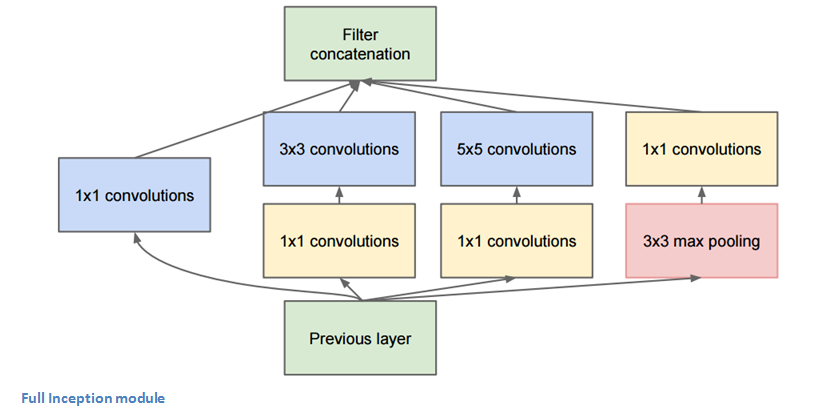
\includegraphics[width=0.7\linewidth]{img/GoogLeNet}
	\label{fig:bloco_inception}
\end{figure}

A Microsoft ResNet foi a CNN vencedora do ILSVRC 2015, com uma taxa de erro top-5 de $3.6\%$. Composta de um total de 152 camadas, esta rede neural deve o sucesso de sua profundidade ao bloco residual, representado na Figura \ref{fig:bloco_residual} que, de maneira resumida, soma à saída de um certo bloco de convoluções a saída de um bloco anterior, para que ambos \emph{feature maps} sejam alimentados à função de ativação ReLU.

\begin{figure}[h!]
\centering
\caption{Bloco Residual da CNN ResNet. Fonte: \cite{torch:resnet}.}\label{fig:bloco_residual}
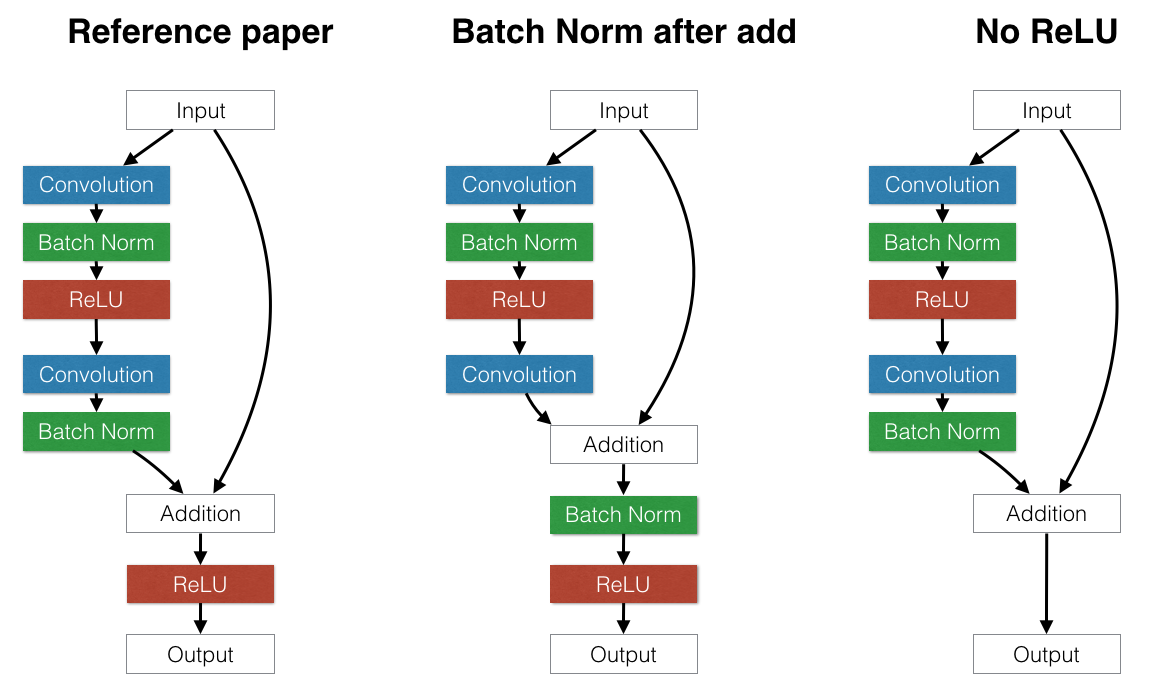
\includegraphics[height=0.3\textheight]{img/resnets_modelvariants}
\end{figure}

Em CNNs tradicionais, a partir de uma imagem de entrada, obtém-se o \emph{feature map} resultante de uma operação de convolução e então aplica-se o \emph{max-pooling}. Este resultado produz uma nova representação, que possui pouca relação com a entrada original. No caso da ResNet, o bloco residual faz com que a entrada original persista em camadas mais profundas da rede, o que garante que as características determinantes para a tarefa de aprendizado sejam disseminadas para camadas mais profundas, ao mesmo tempo em que mantém a dimensionalidade reduzida. Outra razão para o bloco residual ser efetivo é que durante a fase \emph{backwards} o gradiente vai fluir mais facilmente pela rede, pois os blocos residuais estão diretamente conectados às camadas mais rasas na arquitetura, o que facilita a distribuição do gradiente. Na ocasião da sua proposição, a ResNet foi treinada em 8 GPUs por duas a três semanas \cite{resnet}.

Observada a importância das CNNs apresentadas nesta seção, vale notar o esforço computacional para o treino das mesmas, que demora dias mesmo com um hardware específico para este fim. Todo o resultado do treinamento destas redes com o conjunto de dados ImageNet encontram-se disponíveis em \emph{frameworks} para implementação de CNNs, como o  \emph{Keras} \cite{keras:applications} e \emph{Tensorflow} \cite{tensorflow:models}. Disponibilizar estas versões de tais CNNs favorece o aproveitamento das mesmas em contextos análogos, como mostrado a seguir.


\subsection{\emph{Transfer Learning}}
%!TEX root = ../../sbc-template.tex
As várias redes convolucionais treinadas com milhares de exemplos da base de dados  ImageNet e validadas na competição ILSVRC, a exemplo das que foram mencionadas na seção anterior, registram alto desempenho nas tarefas de aprendizado para as quais foram originalmente projetadas. Considerando a arquitetura das mesmas, percebe-se como resultado do treinamento efetuado que uma grande quantidade de parâmetros foi ajustada mediante os milhares de exemplos apresentados, processo este que demorou vários dias mesmo mediante uso de hardware altamente especializado.

Segundo Oquab, representações de imagens aprendidas por CNNs a partir de conjuntos de dados com grande número de exemplos podem ser transferidas eficientemente para outras tarefas de reconhecimento visual que tenham uma quantidade limitada de dados de treinamento \cite{oquab2014learning}. Para tanto, faz-se uso de uma técnica denominada \emph{transfer learning}, que consiste em transferir os conhecimentos entre domínios relacionados. No contexto das CNNs aplicadas em reconhecimento de objetos em imagens, as camadas internas podem agir como detectores de características em médio nível. Estas podem ser pré-treinados na tarefa fonte, na qual utiliza-se um conjunto de dados vasto como o ImageNet, e então re-utilizados na tarefa alvo, que pode conter um conjunto de dados mais restrito.

Após o treinamento para a tarefa original, a rede aprendeu a identificar características mais elementares, como linhas, contornos e objetos, as quais que podem ser redirecionadas na tarefa alvo que possui um objetivo mais específico. O trabalho de Zeiler e Rob, por exemplo, ilustra uma aplicação de \emph{transfer learning}, em que os autores transferem o conhecimento de uma CNN AlexNet treinada originalmente para o conjunto de dados ImageNet adaptando-a para o conjunto de dados Caltech-256, em que a base de dados da tarefa alvo possui apenas cerca de 30 mil imagens a serem usadas numa tarefa de classificação \cite{zeiler2014visualizing}.

Na prática, o \emph{transfer learinng} é feito ao transferir os parâmetros de peso $w$ e de bias $b$ de um modelo já consolidado na literatura e pré-treinado com um conjunto de dados mais robusto, para um modelo similar ainda não treinado. Com o objetivo aproveitar os parâmetros pré-treinados, remove-se a última camada, ou seja, a camada de saída, e em seguida adiciona-se uma ou mais camadas novas, sem treinamento. Neste ponto, outros hiperparâmetros são considerados (número de camadas removidas, quantidade e tipo de camadas adicionadas, por exemplo) e o modelo passa por um processo de ajuste, chamado \emph{fine tuning}, para que ajustar os nossos parâmetros adicionados em conformidade com os pré-existentes, permitindo a extração das características do conjunto de dados da tarefa alvo de maneira satisfatória \cite{oquab2014learning}.



\subsection{Tecnologias Utilizadas}\label{sec:tecs}
%!TEX root = ../../sbc-template.tex

Para a realização deste trabalho são utilizadas tecnologias comumente relacionadas às praticas de ML. A linguagem de programação adotada é o Python 3, em conjunto com bibliotecas como a \emph{Python Data Analysis Library} (Pandas) \cite{pandas} utilizada para análise e consolidação de conjuntos de dados, as bibliotecas de visualização de dados Seaborn \cite{seaborn} e MatPlotLib \cite{matplotlib}, as bibliotecas de ML com suporte a DL Keras \cite{keras} e TensorFlow \cite{tensorflow}. A fim de executar o treinamento e teste dos modelos propostos, utilizou-se uma instância de máquina virtual disponibilizada através da \emph{Google Compute Engine} (GCE) \cite{gce}, dotada de $4$ núcleos de processamento com $4$ GHz cada e $16$ GB de memória RAM. A GCE é parte da \emph{Google Cloud Platform}, uma suíte de computação em nuvem oferecida pelo \emph{Google}.

